%  compress using: gs -sDEVICE=pdfwrite -dCompatibilityLevel=1.4 -dNOPAUSE -dQUIET -dBATCH      -sOutputFile=foo-ShapingSwarmCompressed.pdf ShapingSwarmFrictionSharedInput.pdf

%\documentclass[conference]{IEEEtran}
\documentclass[letterpaper, 10 pt, conference]{ieeeconf}
\IEEEoverridecommandlockouts% This command is only needed if 
                                                          % you want to use the \thanks command
%\overrideIEEEmargins                                      % Needed to meet printer requirements.
\usepackage{times}


\makeatletter 
\let\NAT@parse\undefined
\makeatother

% numbers option provides compact numerical references in the text. 
%\usepackage[numbers]{natbib}
\usepackage{multicol}
\usepackage[bookmarks=true]{hyperref}

\usepackage{bbm}
\usepackage{calc}
\usepackage{url}
\usepackage{transparent}
\usepackage{hyperref}
\hypersetup{
  colorlinks =false,
  urlcolor = black,
  linkcolor = black
}
\usepackage{graphicx}
\usepackage[cmex10]{amsmath}
\usepackage{bm}
\usepackage{amssymb}
\usepackage{rotating}

\usepackage{chngcntr}
\counterwithin{paragraph}{subsection} % makes paragraph depend on subsection


%\usepackage{xfrac}
\usepackage{nicefrac}
\usepackage{cite}
\usepackage[caption=false,font=footnotesize]{subfig}
\usepackage[usenames, dvipsnames]{color}
\usepackage{colortbl}
%\usepackage{caption}

%\usepackage{wrapfig}
\usepackage{overpic}
%\usepackage{subfigure}
%\usepackage{textcomp}
\graphicspath{{./pictures/pdf/},{./pictures/ps/},{./pictures/png/},{./pictures/jpg/}}
\usepackage{breqn} %for breaking equations automatically
\usepackage[ruled]{algorithm}
\usepackage{algpseudocode}
%\usepackage{algorithmic}
\usepackage{multirow}
\usepackage{todonotes}
\usepackage{authblk}

%\newcommand{\todo}[1]{\vspace{5 mm}\par \noindent \framebox{\begin{minipage}[c]{0.98 \columnwidth} \ttfamily\flushleft \textcolor{red}{#1}\end{minipage}}\vspace{5 mm}\par}
% uncomment this to hide all red todos
%\renewcommand{\todo}{}

%% ABBREVIATIONS
\newcommand{\qstart}{q_{\text{start}}}



%% MACROS


\providecommand{\abs}[1]{\left\lvert#1\right\rvert}
\providecommand{\norm}[1]{\left\lVert#1\right\rVert}
\providecommand{\normn}[2]{\left\lVert#1\right\rVert_#2}
\providecommand{\dualnorm}[1]{\norm{#1}_\ast}
\providecommand{\dualnormn}[2]{\norm{#1}_{#2\ast}}
\providecommand{\set}[1]{\lbrace\,#1\,\rbrace}
\providecommand{\cset}[2]{\lbrace\,{#1}\nobreak\mid\nobreak{#2}\,\rbrace}
\providecommand{\lscal}{<}
\providecommand{\gscal}{>}
\providecommand{\lvect}{\prec}
\providecommand{\gvect}{\succ}
\providecommand{\leqscal}{\leq}
\providecommand{\geqscal}{\geq}
\providecommand{\leqvect}{\preceq}
\providecommand{\geqvect}{\succeq}
\providecommand{\onevect}{\mathbf{1}}
\providecommand{\zerovect}{\mathbf{0}}
\providecommand{\field}[1]{\mathbb{#1}}
\providecommand{\C}{\field{C}}
\providecommand{\R}{\field{R}}
\newcommand{\Cspace}{\mathcal{Q}}
\newcommand{\Uspace}{\mathcal{U}}
\providecommand{\Fspace}{\Cspace_\text{free}}
\providecommand{\Hcal}{$\mathcal{H}$}
\providecommand{\Vcal}{$\mathcal{V}$}
\DeclareMathOperator{\conv}{conv}
\DeclareMathOperator{\cone}{cone}
\DeclareMathOperator{\homog}{homog}
\DeclareMathOperator{\domain}{dom}
\DeclareMathOperator{\range}{range}
\DeclareMathOperator{\sign}{sgn}
\providecommand{\polar}{\triangle}
\providecommand{\ainner}{\underline{a}}
\providecommand{\aouter}{\overline{a}}
\providecommand{\binner}{\underline{b}}
\providecommand{\bouter}{\overline{b}}
\newcommand{\D}{\nobreakdash-\textsc{d}}
%\newcommand{\Fspace}{\mathcal{F}}
\providecommand{\Fspace}{\Cspace_\text{free}}
\providecommand{\free}{\text{\{}\mathsf{free}\text{\}}}
\providecommand{\iff}{\Leftrightarrow}
\providecommand{\subinner}[1]{#1_{\text{inner}}}
\providecommand{\subouter}[1]{#1_{\text{outer}}}
\providecommand{\Ppoly}{\mathcal{X}}
\providecommand{\Pproj}{\mathcal{Y}}
\providecommand{\Pinner}{\subinner{\Pproj}}
\providecommand{\Pouter}{\subouter{\Pproj}}
\DeclareMathOperator{\argmax}{arg\,max}
\providecommand{\Aineq}{B}
\providecommand{\Aeq}{A}
\providecommand{\bineq}{u}
\providecommand{\beq}{t}
\DeclareMathOperator{\area}{area}
\newcommand{\contact}[1]{\Cspace_{#1}}
\newcommand{\feasible}[1]{\Fspace_{#1}}
\newcommand{\dd}{\; \mathrm{d}}
\newcommand{\figwid}{0.22\columnwidth}
\newcommand{\TRUE}{\textbf{true}}
\newcommand{\FALSE}{\textbf{false}}
\DeclareMathOperator{\atan2}{atan2}
\allowdisplaybreaks

\newtheorem{theorem}{Theorem}
\newtheorem{definition}[theorem]{Definition}
\newtheorem{lemma}[theorem]{Lemma}


\pdfinfo{
   /Author (Shiva Shahrokhi, Chris Ertel and Aaron T. Becker)
   /Title  (Controlling a Swarm With Global Inputs: Varying Controller Type )
   /CreationDate (D:20160129120000)
   /Subject (Simple Robots)
   /Keywords (Robots;Uniform Control Inputs)
}


% paper title
\title{\LARGE \bf Controlling a Swarm With Global Inputs: Varying Controller Type}

% You will get a Paper-ID when submitting a pdf file to the conference system
\author{Shiva Shahrokhi, Chris Ertel and Aaron T. Becker% <-this % stops a space
\thanks{*This work was supported by the National Science Foundation under Grant No.\ \href{http://nsf.gov/awardsearch/showAward?AWD_ID=1553063}{ [IIS-1553063]} and \href{http://nsf.gov/awardsearch/showAward?AWD_ID=1619278}{[IIS-1619278]}.}% <-this % stops a space
\thanks{Authors are with the Department of Electrical and Computer Engineering,  University of Houston, Houston, TX 77204 USA        {\tt\small  \{sshahrokhi2, atbecker\}@uh.edu}}%
}
%\affil{Department of Electrical and Computer Engineering, \\
% University of Houston, Houston, TX 77204-4005 USA\\
% {\tt\small  \{sshahrokhi2, aviswanathanmahadev, atbecker\}@uh.edu}}
%\thanks{S. Shahrokhi, A. Mahadev and  A. Becker are with the Department of Electrical and Computer Engineering,  University of Houston, Houston, TX 77204-4005 USA {\tt\small  \{sshahrokhi2, aviswanathanmahadev, atbecker\}@uh.edu}
%}
%} %\end thanks

\begin{document}



\maketitle
\thispagestyle{empty}
\pagestyle{empty}


\begin{abstract}
There are driving applications for large populations of tiny robots in robotics, biology, and chemistry.
These robots often lack onboard computation, actuation, and communication.
Instead, these ``robots''  are  particles carrying some payload and the particle swarm is controlled by a shared, global control input such as a uniform magnetic gradient or electric field.
Different controller types are used. Repulsive and attractive controllers are the 
Requiring a small, rigid obstacle suspended in the middle of the workspace is a strong constraint, especially in 3D.
%Often particles are placed into an em
This paper relaxes that constraint, and provides position control algorithms that only require interactions with the boundaries.
Both in vivo and artificial environments often have boundaries.
We assume that particles in contact with the boundaries have zero velocity if the global control input pushes the particle into the wall.
This paper provides a shortest-path algorithm for positioning a two-particle swarm, and a generalization to positioning an $n$-particle swarm.
Results are validated with simulations and a hardware demonstration.







%Consider a swarm of particles controlled by global inputs. 
%This paper presents algorithms for shaping such swarms in 2D using boundary walls.
%The range of configurations created by conforming a swarm to a boundary wall is limited. 
%We describe the set of stable configurations of a particle swarm in two canonical workspaces, a circle and a square. 
%To increase the diversity of configurations, we add boundary interaction to our model.  
%We provide algorithms using friction with walls to place two robots at arbitrary locations in a rectangular workspace.
%Next, we extend this algorithm to place $n$ agents at desired locations. 
%We conclude with efficient techniques to generate correlations of a particle swarm not possible without wall-friction. 
%Simulations %and hardware implementations with 100 robots 
%validate these results.

%These methods may have particular relevance for micro- and nano-robots controlled by global inputs.
%, whose small size limits onboard computation and power. For this reason they are usually powered and controlled by global inputs, such as a uniform external electric or magnetic field, and every robot receives the same control inputs.
%Due to their small size, large numbers of micro-robots are required to deliver sufficient payloads.
% Nevertheless, these applications require precision control of the shape and position of the robot swarm. Precision control requires breaking the symmetry caused by the global input.  

 



% KEYWORDS:   uniform control, under-actuation, particle swarm
\end{abstract}

\IEEEpeerreviewmaketitle

%%%%%%%%%%%%%%%
%\section{Introduction}\label{sec:Intro}

This chapter investigates maximizing torque applied by a large number of particles, hereafter called a \emph{swarm}, when the swarm has non-slip contact with a rigid, 2D body. 
 The under-actuated swarm is steered by a shared signal that consists of a vector direction for movement. 
  The robotic system is comprised of the swarm of particles, the shared control signal, and an external sensor that measures the swarm position.
   This chapter examines analytically two representative aspects of swarm torque control: first, pushing a pivoted rod, and second pushing a free body. 
   We conclude with hardware experiments with centimeter-scale robots. Maximizing torque improves the efficiency of a particle swarm.

 

\begin{figure}
\begin{center}
	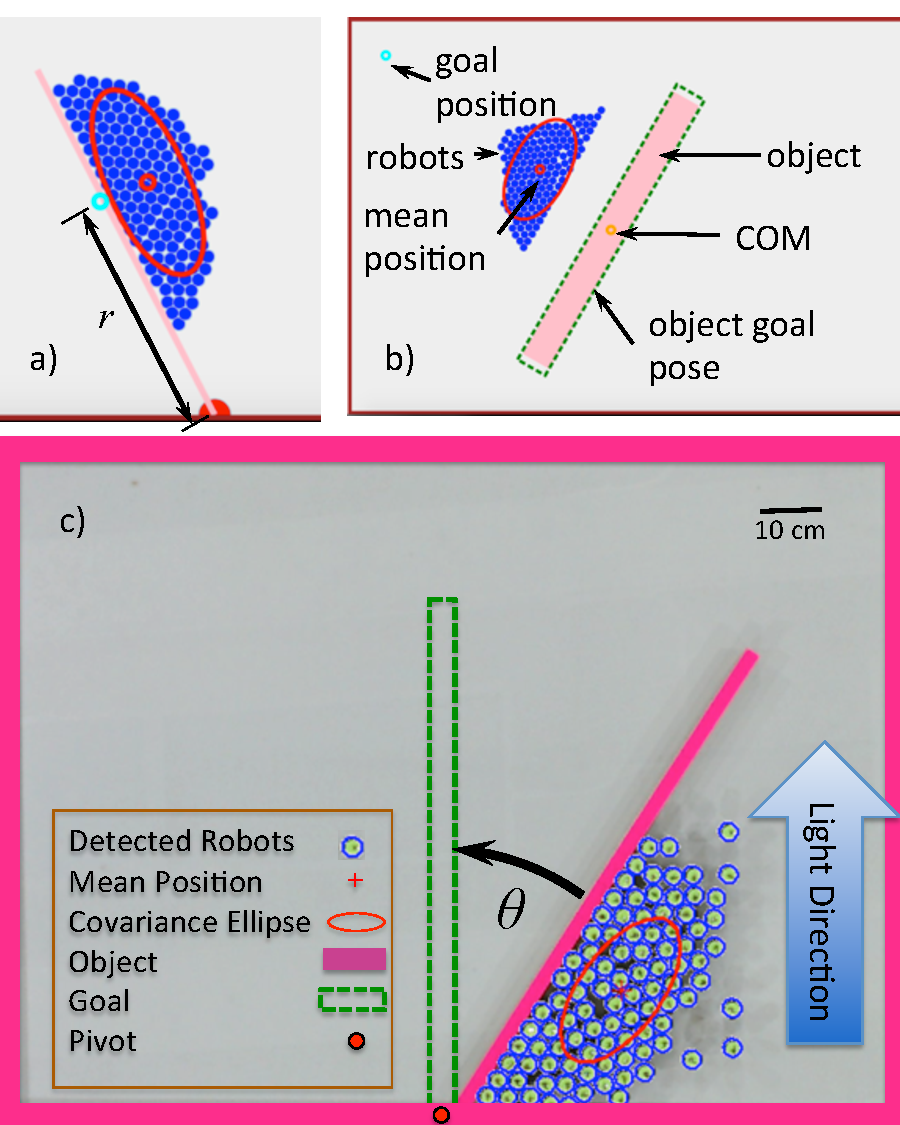
\includegraphics[width=.9\columnwidth]{CoverPhoto.pdf}
\end{center}
\vspace{-1em}
\caption{\label{fig:FirstImage}
%Torque control of an object is essential for manipulation unless objects are homogeneous discs, especially when there are narrow passageways or the objects must be aligned, e.g. sensors and emitters. 
%This paper provides the optimal position for a swarm to push to maximize torque production using a highly under-actuated system where all robots are controlled uniformly by the same input. 
(a) Simulation of robots exerting torque on a hinged ``door".
(b) Orientation control of a free long rod.
(c) Hardware robots applying torque to an object. See video attachment.% A full resolution video is available at \url{https://youtu.be/7Q5lu_ZFbxI}.
}
\vspace{-1em}
\end{figure}

With a single agent, torque control is straightforward: the agent simply maximizes the length of the movement arm to maximize torque. To make an agent push open a door, it should push on the edge furthest from the hinge. 
The optimal solution for a swarm of particles is not straightforward because they cannot all push at one position.

This chapter focuses on maximizing torque using the swarm's position distribution. 
Representative results are shown in Fig. \ref{fig:FirstImage}:  torque control using 56 mobile robots on a pivoted and a free object.




%%%%%%%%%%%%%%%
%%%%%%%%%%%%%%%
%
%%%%%%%%%%%%%%%%%%%%%%%%%%%%%%%%%%%%%%%%%%%%%%%%%%%%%%%%%%%
\section{Related work}\label{sec:RelatedWork}
%%%%%%%%%%%%%%%%%%%%%%%%%%%%%%%%%%%%%%%%%%%%%%%%%%%%%%%%%%%

Controlling the \emph{shape}, or relative positions, of a swarm of robots is a key ability for a range of applications.  Correspondingly, it has been studied from a control-theoretic perspective in  both centralized and decentralized approaches. For examples of each, see the centralized virtual leaders in \cite{egerstedt2001formation}, and the  gradient-based decentralized controllers  using control-Lyapunov functions in~\cite{hsieh2008decentralized}. However, these approaches assume a level of intelligence and autonomy in individual robots that exceeds the capabilities of many systems, including current micro- and nano-robots.  Current micro- and nano-robots, such as those in~\cite{Chowdhury2015,martel2015magnetotactic,Xiaohui2015magnetiteMicroswimmers} lack onboard computation.

This chapter focuses on centralized techniques that apply the same control input to both particles. 
Precision control requires breaking the symmetry caused by the uniform input.  
Symmetry can be broken using particles that respond differently to the uniform control signal, either through agent-agent reactions \cite{bertozzi2015ring}, or engineered inhomogeneity  \cite{Donald2013,bretl2007,beckerIJRR2014}. 
 The magnetic gradients of MRI scanners are \emph{uniform}, meaning the same force is applied everywhere in the workspace\cite{nosrati2018development}.
 This work assumes a uniform control with homogenous particles, as in~\cite{AaronManipulation2013}, and breaks the control symmetry using obstacles in the workspace. 

%The techniques in this paper are inspired by artificial force-fields. 

%\emph{Fluid-flow:} 
%Fluid flow along boundaries generates a shear force that pushes different parts of a body in opposing directions. 
%Most introductory fluid dynamics textbooks provide models~\citep{Munson2013}.
%Similarly, a swarm of robots under global control pushed along a boundary will experience shear forces.  
%This is a position-dependent force, and so can be exploited to control the configuration or shape of the swarm.  
% \citep{spears2006physics}~used these forces to disperse a swarm's spatial position for coverage for physics-based swarm simulations.

%\emph{Artificial Force-fields:}
%Much research has focused on generating non-uniform artificial force-fields that can be used to rearrange passive components. 
Alternative techniques rely on non-uniform inputs, such as artificial force-fields.
Applications have included techniques to design shear forces for sensorless manipulation of a single object by~\cite{lamiraux+2001:ra}.  
\cite{vose2012sliding} demonstrated a collection of 2D force fields generated by six degree-of-freedom vibration inputs to a rigid plate.  These force fields, including shear forces, could be used as a set of primitives for motion control to steer the formation of multiple objects. %However unlike the uniform control model in this paper, their control was multi-modal and position-dependent.
%\todo{talk about obstacles, think about adding goldberg}

%This paper develops control algorithms using uniform control fields, such as the magnetic resonance navigation \cite{nosrati2018development}.%field in a clinical MRI [insert a recent reference from Sylvain Martel using MRI].
Similarly, much recent work in magnet control has focused on exploiting inhomogeneities in the magnetic field to control multiple micro particles  using gradient-based pulling~\cite{Salmanipour2018EightDOF,Denasi2018independent}.  
Unfortunately, using large-scale external magnetic fields makes it challenging to independently control more than one microrobot unless the  distance between the electromagnetic coils is at the same length scales as the robot workspace~\cite{diller2016six, Denasi2018independent, Salmanipour2018EightDOF }. In contrast, % to methods that exploit inhomogeneities in the magnetic field to control multiple micro particles, e.g. \cite{Denasi2018independent}, that exploited nonlinearities generated by four magnetic coils in close proximity to the workspace to achieve trajectory control of two microspheres, 
 this chapter requires only a controllable constant gradient in orthogonal directions to position the particles.
% Systems like this one are poorly suited for PRM and RRT*-type methods\cite{lavalle2006planning} because if during a movement a collision occurs, that movement is irreversible.
   %Flow in a pipe or body lume

If a control input causes the particles to collide with obstacles at different times, inverting the control input does not undo the action. 
 Due to this lack of time-reversibility, techniques that require a bidirectional graph, e.g. PRM \cite{kavraki1996probabilistic} and RRT* \cite{lavalle2006planning} are not suitable.
  Instead, this chapter employs a greedy search strategy. 
%%%%%%%%%%%%%%%
%%%%%%%%%%%%%%%
%%%%%%%%%%%%%%%%%%%%%%%%%%%%%%%%%%%%%%%%%%%%%%%%%%%%%%%%%%%
\section{Online experiment}
\label{sec:expMethods}
%%%%%%%%%%%%%%%%%%%%%%%%%%%%%%%%%%%%%%%%%%%%%%%%%%%%%%%%%%%

% Experimental Methods
%%  Platform  
%%  Human Subjects
%%% recruited through social media
%%% IRB form  Protocol Number: 14-012E Protocol Title: Massive Manipulation: A n online user study on controlling large swarms of simple robot sApproval Date: 7/26/2013Expiration Date: 7/26/2014
%%% Costs  for experiment:  ??
%%% Instrumenting:
%%%% Google analytics, airbrake, etc.

%% wherein we describe our framework


We have developed a flexible testing framework for online human-swarm interaction studies. 
%There are two halves to our framework: the server backend and the client-side (in-browser) frontend. The server backend is responsible for tabulating results, serving webpages containing the frontend code, and for issuing unique identifiers to each experiment participant. The in-browser frontend is responsible for running an experiment---that is to say, accepting user input, updating the state of the robot swarm, and ultimately evaluating task completion.

%% wherein we outline the process that a user takes to participate in an experiemnt
\subsection{Methods}

%\paragraph{Overview}

A participant visits the site, initiating a communication between their browser and our server. The web server generates a unique identifier for the participant and sends it along with the landing page to the participant---this identifier is stored as a browser cookie and will be sent along with all results the participant generates. 
%The participant's browser prompts for confirmation of the terms-of-service and offers a menu of experiments.

%Once the participant selects an experiment, their browser makes a new request to the server to load the experiment's webpage. The server sends scaffold HTML describing the layout of the page and a script block containing the experiment. 
The script runs the experiment and, upon a successful completion, posts the experiment data to the server. 
%The participant is then given the option of playing again or trying a different experiment.

A participant may view all of the experimental data we have gathered; this information is available as either a webpage, a JSON file, or a comma-separated value file.

%% wherein we preach the good word of Ruby and describe what the backend actually does
%\paragraph{Backend}

%The server backend is written in Ruby, using the Ruby-on-Rails (abbreviated \emph{Rails}) web development framework. Ruby is a dynamically-typed object-oriented scripting language with a strong emphasis on programmer ergonomics and metaprogramming support. It is well-suited for the creation of domain-specific languages for a variety of tasks, as exemplified by the Rails framework. Our backend serves assets (images, scripts, stylesheets, and so forth) to participants, selects the correct script to send to perform a particular experiment, and stores results.

%Each result is a database record containing the experiment name, the participant identifier, the duration of the experiment (time to completion), the number of robots involved, the detailed mode information of the experiment, and the user agent string of the browser running the experiment (which identifies the type of browser used by the participant). Rails automates the process of creating the relevant database-object bindings, and thus we spent little time creating or modifying the result records, allowing us to rapidly adapt the server to our needs--for example, adding tracking of the user agent and experiment mode both took less than five minutes of work on the server side.

%The experiment script file to be sent to the client is chosen with the uniform resource identifier (URI) for the experiment webpage; this done, the server will render the page requested by the participant and insert the script for the selected experiment. The Rails framework has a great deal of support for optimizing and compacting (\emph{minifying}) Javascript files.

%% wherein we decry the evils of javascript and explain why we use the browser
%\paragraph{Frontend}

%The client frontend which runs in the participant's browser is written in Javascript, a dynamically-typed prototype-oriented scripting language with some functional programming support. We make heavy use of the Underscore framework (a functional programming toolkit for Javascript) as well as the Javascript port of \href{http://box2d.org/}{Box2D} (a popular 2D physics engine with good support for rigid-body dynamics and fixed-timestep simulation). Our frontend also includes helper libraries for drawing robots, handling user input, and drawing graphs.

%Our framework uses a base task to represent the lifecycle of an experiment---{\bf  instantiation, simulation, evaluation}, and {\bf submission}. A particular experiment inherits from this prototype but overrides particular methods and adds its own variables for bookkeeping; this allows new or modified tasks to be created rapidly with minimal boilerplate code.

%\paragraph{Model}
%Our robots are disc-shaped, non-holonomic, and confined to the 2D plane.  The control input $u$ consists of a single bounded force vector that is applied to each robot, $|u|\le u_{max}$.  We include a linear ramp for this force value that starts at zero and increases to the maximum value in one second; this allows participants to do fine control of the robots by tapping the arrow keys.
%\begin{align}\label{eq:sysmodel}
%\dot{x}_i = u_x,  \qquad  \dot{y}_i = u_y.
%\end{align}

During the {\bf instantiation} phase, an experiment sets up the web page elements with help text and other information, and creates the obstacles, robots, and workpieces that will be present during the experiment. It will also randomly select which mode to run in, if applicable.

The {\bf simulation} phase is the time at which all of the robots are moved according to user input and given a chance to interact with each other and the environment. The simulation phase then draws the current state of the experiment to the canvas of the webpage.

The {\bf evaluation} phase is when the experiment's completion criteria are applied to the current experiment state: are the robots in the goal zone, are the workpieces in the correct place, and so forth. If the criteria are not met, the experiment loops back into the simulation phase; if they are met, then the experiment proceeds to result submission.

The {\bf submission} phase is when the results of the experiment are combined with other user data, such as the browser user agent string, and submitted to the server for collection.

%As a means of encouraging user interaction, the results of other runs of the experiment are shown to the participant after submission along with merit badges displaying the number of experiments completed.

%% wherein we justify hours spent on facebook and hacker news  -- ha!  I'd like us to place links in the .tex for future reference
\paragraph{Human subjects:}
Because our study involved recording data from human subjects, it required IRB approval before we could legally save user data (IRB \#14357-01).
%% IRB form  Protocol Number: 14-012E Protocol Title: Massive Manipulation: An online user study on controlling large swarms of simple robot sApproval Date: 7/26/2013Expiration Date: 7/26/2014
%Rice Federal-Wide Assurance Number: 00003890

%Subjects were recruited using a combination of social network effects and coordinated news posts. We asked our friends and colleagues to send links to our site to their friends via their preferred social networks, generally Twitter, Facebook, Google+, and through email. Additionally, we posted our site to several news aggregators in hopes that it would be seen and visited. Our first such posting was to \href{https://news.ycombinator.com/item?id=6277052}{Hacker News}, an aggregator run by the Y-Combinator accelerator company; this posting resulted in our first thousand trials. A second posting was made to Reddit, but did not seem to cause much traffic. A third posting was made to the  \href{http://robohub.org/researchers-use-single-joystick-to-control-swarm-of-rc-robots/}{Robohub.org} site. The traffic generated by these postings is shown in Fig.~\ref{fig:timePlayed}. 

\begin{figure}
\centering
\begin{overpic}[width = .5\columnwidth]{timePlayed.pdf}\end{overpic}
\vspace{-2em}
\caption{
\label{fig:timePlayed}
Cumulative time played for completed tests.
}
%\vspace{-2em}
\end{figure}


%Concurrently, we contacted our university's  \href{http://news.rice.edu/contact-us/}{\emph{News and Media Relations Team}}. They sent a writer and photographer to our lab, worked with us to draft a \href{http://news.rice.edu/2013/09/09/a-swarm-on-every-desktop-robotics-experts-learn-from-public/ }{press release}, and publicized with news outlets and alumni. Most universities have a media team, and this is a valuable no-cost resource to gain publicity.
 
%% wherein we show just how cheap we are 
%\subsubsection{Experimental costs}

%We've spent approximately one hundred dollars USD provisioning and running this experiment. Hosting is provided by \href{Heroku.com}{Heroku}, using a single web instance costing around \$40/month, with additional monitoring services bringing that up to \$50/month. In the event of increased demand/participant traffic, we can provision another server to take up the load.
%We purchased our domain name from \href{Namecheap.com}{Namecheap.com} for \$11.66 a year, giving our site a short, easy to pronounce handle.
%SwarmControl.net %16 char
%SwarmControl.herokuapp.com %26 char

%As mobile traffic becomes more prominent and overtakes the volume of internet access from desktop computers & laptops, shorter domain names will become increasingly more important and more desirable.  The likelihood of a typo on a mobile device is increased and that  can be hedged by having a shorter domain name which requires less typing and fewer characters to enter. - See more at: http://www.mediaoptions.com/domain-names/short-is-sweet-the-value-of-short-domain-names.html#sthash.AJNqlXhB.dpuf

%Given the large number of experiment sessions run (over 11,000 at the time of this writing), we see a per-experiment cost of less than three cents.

%% wherein we describe how we monitor the progress of the experimental setup
%\subsubsection{Instrumentation}

%When conducting an online experiment, it is helpful to gather data about both the experiment infrastructure and the participants. For the backend, we use a service called Airbrake to monitor the Rails server, getting emails in the events of any errors occurring or suspicious activity. We also use another service called New Relic to provide monitoring and analytics on the server traffic, giving coarse statistics about site visitation, page load time, and other indicators of how our backend is performing.

%For the frontend, we use Google Analytics to track user behavior. This tool allows us to see country of origin for users, time spent on the site, relative percent of people who look past the landing page (bounce rate), and user agent information (type of browser, type of device, etc.).


%%%%%%%%%%%%%%%%%%%%%%%%%%%%%%%%%%%%%%%%%%%%%%%%%%%%%%%%%%%
\subsection{Human-swarm interaction results}\label{sec:expResults}
%%%%%%%%%%%%%%%%%%%%%%%%%%%%%%%%%%%%%%%%%%%%%%%%%%%%%%%%%%%

We designed six experiments to investigate human control of large robotic swarms for manipulation tasks.  Screenshots of each experiment are shown in Fig.~\ref{fig:5experiments}.  Each experiment examined the effects of varying a single parameter: population of robots for manipulation, four levels of visual feedback, different levels of Brownian noise, position control with 1 to 10 robots, and three control architectures for both an assembly task and a foraging task. The users could choose which experiment to try, and then our architecture randomly assigned a particular parameter value for each trial.  We recorded the completion time and the participant ID for each successful trial.  
%As Fig.~\ref{fig:Learning} shows, one-third of all participants played only a single game.  Still, many played multiple games, and their decreasing completion times demonstrates their skills improved.


\paragraph{Varying number}
\begin{figure}
\begin{overpic}[width = 0.5\columnwidth]{ResVaryNum.pdf}\end{overpic}
\begin{overpic}[width = 0.48\columnwidth]{measureLearning.pdf}\end{overpic}
\caption{
\label{fig:ResVaryNu}Data from \emph{Varying Number} using robots to push an object through a maze to a goal location.  (Left) Data indicates this task has an optimal number of robots, perhaps due to the relative sizes of the robots, obstacles, and object. Best-fit linear and quadratic lines are overlaid for comparison. 
(Right) Skill improves as players retry tests using data from \emph{Varying Number}.
}
\end{figure}



Transport of goods and materials between points is at the heart of all engineering and construction in real-world systems. This experiment varied from 1 to 500 the population of robots used to transport an object. The total area, maximum robot speed, and total net force the swarm could produce were constant. The robots pushed a large hexagonal object through an  {\sffamily S}-shaped maze. We hypothesized participants would complete the task faster with more robots. The results, shown in Fig.~\ref{fig:ResVaryNu}, do not support our hypothesis, indicating a minima around 130 robots.



\paragraph{Varying visualization}
\begin{figure}[b!]
\renewcommand{\figwid}{0.24\columnwidth}
\begin{overpic}[width =\figwid]{VaryVisFS.pdf}\put(20,15){Full-state}\end{overpic}
\begin{overpic}[width =\figwid]{VaryVisCH.pdf}\put(10,15){Convex-hull}\end{overpic}
\begin{overpic}[width =\figwid]{VaryVisMV.pdf}\put(10,15){Mean + var}\end{overpic}
\begin{overpic}[width =\figwid]{VaryVisMe.pdf}\put(30,15){Mean}\end{overpic}
\vspace{-.5em}
\caption{\label{fig:Visualization}Screenshots from task \emph{Vary Visualization}. This experiment challenges players to quickly steer 100 robots (blue discs) to push an object (green hexagon) into a goal region. We record the completion time and other statistics.
%\vspace{-1em}
}
\end{figure}

\begin{wrapfigure}{R}{0.5\textwidth}
  \vspace{-20pt}
  \begin{center}
  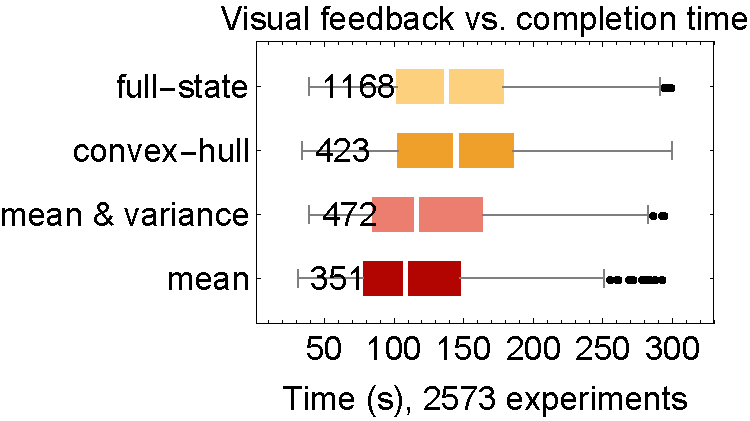
\includegraphics[width=0.5\textwidth]{ResVaryVis.pdf}
  \end{center}
  \vspace{-1em}
\caption{\label{fig:ResVaryVis} Completion-time results for the four levels of visual feedback shown in Fig.~\ref{fig:Visualization}.  Players performed better with limited feedback.
\vspace{-1em}
}
\end{wrapfigure}

Sensing is expensive, especially on the nanoscale. To see nanocars~\cite{Chiang2011} fastened molecules that fluoresce light when activated by a strong light source. Unfortunately, multiple exposures can destroy these molecules, a process called \emph{photobleaching}. Photobleaching can be minimized by lowering the excitation light intensity, but \cite{Cazes2001} showed this increases the probability of missed detections.  This experiment explores manipulation with varying amounts of sensing information: {\bf full-state} sensing provides the most information by showing the position of all robots; {\bf convex-hull} draws a convex hull around the outermost robots; {\bf mean} provides the average position of the population; and {\bf mean + variance} adds a confidence ellipse. Fig.~\ref{fig:Visualization} shows screenshots of the same robot swarm with each type of visual feedback. Full-state requires $2n$ data points for $n$ robots. Convex-hull requires at worst $2n$, but according to \cite{har2011expected}, the expected number is $O(2 n^{1/3})$.  Mean requires two, and variance three, data points.  Mean and mean + variance are convenient even with millions of robots. 

%\begin{figure}[b!]
%\renewcommand{\figwid}{0.5\columnwidth}
%\begin{overpic}[width =\figwid]{ResVaryVis.pdf}\end{overpic}
%\vspace{-1em}
%\caption{\label{fig:ResVaryVis} Completion-time results for the four levels of visual feedback shown in Fig.~\ref{fig:Visualization}.  Players performed better with limited feedback.
%%\vspace{-1em}
%}
%\end{figure}




% Additionally, as population characteristics, they are available even if only a percentage of the robots are detected each control cycle.
%Photobleaching: http://www.piercenet.com/browse.cfm?fldID=4DD9D52E-5056-8A76-4E6E-E217FAD0D86B
%
%Photobleaching is caused by the irreversible destruction of fluorophores due to either the prolonged exposure to the excitation source or exposure to high-intensity excitation light. Photobleaching can be minimized or avoided by exposing the fluor(s) to the lowest possible level of excitation light intensity for the shortest length of time that still yields the best signal detection; this requires optimization of the detection method using high sensitivity CCD cameras, high numerical aperture objective and/or the widest bandpass emission filter(s) available. Other approaches include using fluorophores that are more photostable than traditional fluorophores and/or using antifade reagents to protect the fluor(s) against photobleaching. Steps to avoid photobleaching are not feasible for all detection methods and should be optimized for each method used. For example, antifade reagents are toxic to live cells, and therefore they can only be used with fixed cells or tissue. Furthermore, some detection methods, such as flow cytometry, normally do not require steps to avoid photobleaching because of the extremely short exposure time of the fluorophore to the excitation source.


%\begin{figure}
%\centering
%\begin{overpic}[width = \columnwidth]{ResVaryVis.pdf}\end{overpic}
%\vspace{-2em}
%\caption{\label{fig:ResVaryVis} Completion-time results for the four levels of visual feedback shown in Fig.~\ref{fig:Visualization}. Surprisingly, players perform better with limited feedback--subjects with only the mean + variance  outperformed all others.
%\vspace{-2em}
%}
%\end{figure}

Our hypothesis predicted a steady decay in performance as the amount of visual feedback decreased.
Our experiment indicated the opposite: players with just the mean completed the task faster than those with full-state feedback.  As Fig.~\ref{fig:ResVaryVis}.b shows, the levels of feedback arranged by increasing completion time are [ mean, mean + variance, full-state, convex-hull].  All experiments lasting over 300s were removed, under the assumption that the user stopped playing. 
Using ANOVA analysis, we reject the null hypothesis that all visualization methods are equivalent, with $p$-value $2.69\times10^{-19}$.
Anecdotal evidence from beta-testers who played the game suggests that tracking 100 robots is overwhelming---similar to schooling phenomenons that confuse predators---while working with just the mean + variance is like using a ``spongy'' manipulator. Our beta-testers described convex-hull feedback as confusing and irritating.  A single robot left behind an obstacle will stretch the entire hull, obscuring the majority of the swarm.
%obscuring what the rest of the swarm is doing.   

\paragraph{Varying noise}
Microrobots are affected by random collisions with molecules. The effect of these collisions is called Brownian motion.

This experiment varied the strength of these disturbances to study how noise affects human control of large swarms. Noise was applied at every timestep as follows:
\begin{align*}
\dot{x}_i &= u_x + m_i\cos(\psi_i)\\
 \dot{y}_i &= u_y + m_i\sin(\psi_i).
 \end{align*}
$m_i,\psi_i$ are uniformly IID, with $m_i\in[0,M]$ and $\psi_i\in[0,2\pi]$. $M$ is a constant for each trial ranging from 0 to 200\% of the maximum control power ($u_{max}$).
 
We hypothesized 200\% noise was the largest a human could be expected to control---at 200\% noise, the robots move erratically.  Disproving our hypothesis, the results in Fig.~\ref{fig:ResVaryNoisePosition}.a show only a 40\% increase in completion time for the maximum noise.

\begin{figure}[b!]
\renewcommand{\figwid}{0.5\columnwidth}
\begin{overpic}[width =\figwid]{ResVaryNoise.pdf}\end{overpic}
\begin{overpic}[width =\figwid]{ResPositioning.pdf}\end{overpic}
\vspace{-1em}
\caption{\label{fig:ResVaryNoisePosition} Left: Varying the noise from 0 to 200\% of the maximum control input resulted in only a small increase in completion time. Right: Increasing the number of robots resulted in longer completion times.  For more than 4 robots the goal pattern contained a void, which may have caused the jump in completion times.
%\vspace{-1em}
}
\end{figure}


\paragraph{Position control}
This online experiment examined how completion time scales with the number of robots $n$. Using a single square obstacle, users arranged $n\in[1,10]$ robots into a specified goal pattern.  The goal pattern formed a block  {\sffamily A} with 10 robots, and lesser numbers of robots used a subset of these goal positions. Our hypothesis was that completion time would increase linearly with the number of robots, as with our position control algorithm in \cite{Becker2013b}.  Our results roughly corroborate this, as shown in Fig.~\ref{fig:ResVaryNoisePosition}.b.  Though the number of robots presented to game players is uniformly distributed, larger $n$ are more difficult, and the number of successful experiments drops steadily as $n$ increases.



Note there is a bifurcation between $n$=4 and $n$=5 robots. For $n\in[1,4]$ the goal patterns are not hollow, but starting at $n$=5 they are.  A better experiment design would randomly place the goal positions.  Initially we tried this, but our beta-testers strongly disliked trying to arrange robots in random patterns.


\paragraph{Varying control: Assembly}
Ultimately, we want to use swarms of robots to build things. This experiment compared different control architectures modeled after real-world devices.

We compared attractive and repulsive control with the global control used for the other experiments. The attractive and repulsive controllers were loosely modeled after scanning tunneling microscopes (STM), but also apply to magnetic manipulation, e.g.\ \cite{Khalil2013} and biological models, e.g. \cite{goodrich2012types}. STMs can be used to arrange atoms and make small assemblies, as described in \cite{avouris1995manipulation}. An STM tip is charged with electrical potential, and used to repel like-charged or to attract differently-charged molecules. In contrast, the global controller uses a uniform field (perhaps formed by parallel lines of differently-charged conductors) to pull molecules in the same direction.
The experiment challenged players to assemble a three-block pyramid with a swarm of 16 robots.

%\todo{describe controller model here, use an equation}

The results were conclusive, as shown in Fig.~\ref{fig:ResVaryControl}.a: attractive control was the fastest, followed by global control, with repulsive control a distant last.  The median time using repulsive control was four times longer than with attractive control.
Using ANOVA analysis, we reject the null hypothesis that all controllers are equivalent, with $p$-value $3.37\times10^{-32}$.

%%\begin{figure}
%%\begin{overpic}[width = 0.39\columnwidth]{attractiveForce.pdf}\end{overpic}
%%\begin{overpic}[width = 0.6\columnwidth]{understandingForces.pdf}\end{overpic}
%%\caption{
%%\label{fig:attractiveForce}
%%Attraction and repulsion with a point source distance $h$ above the plane and $r$ from the robot. 
%%}
%%\end{figure}

\begin{figure}[b!]
\renewcommand{\figwid}{3.3cm}
\begin{overpic}[height =\figwid]{ResVaryControl.pdf}\end{overpic}
\begin{overpic}[height =\figwid]{ResVaryForage.pdf}\end{overpic}
\vspace{-.5em}
\caption{\label{fig:ResVaryControl} Completion time depends on both the task and the control type. Left: Attractive control resulted in the shortest completion time and repulsive the longest for building a three-block pyramid. Right: in the foraging test, global control resulted in the shortest completion time and attractive the longest.
%\vspace{-1em}
}
\end{figure}

\paragraph{Varying control: Foraging}
Collecting and delivering resources is necessary for drug delivery.
This experiment also compared attractive and repulsive control with the global control used for the other experiments. The experiment challenged players to collect particles using a swarm of 100 robots and return the particles to a home region. The robots encapsulate the particles on contact. 

%\todo{describe controller model here, use an equation}

The results were conclusive, as shown in Fig.~\ref{fig:ResVaryControl}.b: global control was the fastest, followed by repulsive control, with attractive control last.  Using ANOVA analysis, we reject the null hypothesis that all controllers are equivalent, with $p$-value $2.96\times10^{-6}$.



%%%%%%%%%%%%%%
%%%%%%%%%%%%%%
%%%%%%%%%%%%%%%%%%%%%%%%%%%%%%%%%%%%%%%%%%%%%%%%%%%%%%%%%%%%
\section{Experimental Results}\label{sec:expResults}
%%%%%%%%%%%%%%%%%%%%%%%%%%%%%%%%%%%%%%%%%%%%%%%%%%%%%%%%%%%
\begin{figure*}[htb!]\label{fig:3dPrinted}
\centering
\vspace{1.5em}
%\begin{overpic}[width=\columnwidth]{firstImage.jpg}\end{overpic}
\begin{overpic}[width=2\columnwidth]{3dexperiment.pdf}\end{overpic}
\\
\vspace{1em}
\begin{overpic}[width=2\columnwidth]{realTripe.pdf}\end{overpic}
\caption{\label{fig:story}
Frames showing particle positions before and after control inputs. Top row: small intestine phantom. Bottom row: cow stomach tissue.
} \vspace{-1em}
\end{figure*}

To demonstrate Alg.~\ref{alg:optimalAlg} experimentally, we performed several tests.
Each used the same magnetic setup shown in Fig.~\ref{fig:IntroPic}.
% The figure might need to be referenced 
 Two different intestine models were employed, the first a 3D-printed cross-section representation of a small intestine, and the second a cross-section of a bovine stomach.
 
 \subsection{Magnetic Manipulation Setup}
 
 The magnetic manipulation system has two pairs of electromagnetic coils, each with iron cores at their centers, and arranged orthogonal to each other. The iron core at the center of each coil concentrates the magnetic field towards the workspace. An Arduino and four SyRen regenerative motor drivers were used for control inputs to the coils. Finally, a FOculus F0134SB 659 x 494 pixel camera was attached to the top of the system, focusing on the workspace which was backlit by a $\SI{15}{\watt}$ LED light strip. 
 
To obtain experimental data, the test samples (the phantom intestine model and the bovine cross section) were placed in laser-cut acrylic discs and then immersed in corn syrup. Corn syrup was used to increase the viscosity to 12000 cP for the experiments. Spherical $\SI{1}{\milli\metre}$ magnets (supermagnetman \#SP0100-50) were used as our particles. Our experimental setup did not perfectly implement the system dynamics in \eqref{eq:swarmDynamicsAndFric}. In particular, the magnetic field in this setup is only approximately uniform. The magnetic force varies in both magnitude and orientation. As shown in the video attachment, this non-uniformity causes the particle closer to the coil to move faster than the other particle. This phenomenon makes it easier to increase particle separation than to decrease separation, but this can be compensated because boundary collisions easily decrease the separation. Also, magnetic forces are not exactly parallel, but point toward the center of the activated coil. Algorithm~\ref{alg:optimalAlg} still works despite these non-uniformities, but sometimes requires additional iterations.
 
%explain the magnetic field strength used, the camera system (briefly)
%explain the particles used

%explain the fluid used in the model.

\subsection{Intestine Phantom Model}

The intestine phantom model was used first and was made to mimic the geometry of an intestine and its villi. The model consists of a circular ring with an outer diameter of $\SI{50}{\milli\metre}$, an inner diameter of $\SI{46}{\milli\metre}$, and 60 $\SI{2}{\milli\metre}$ long protrusions on its inner surface cut out of $\SI{6}{\milli\metre}$ thick acrylic to model the geometry of intestinal villi. Figure \ref{fig:story} top row shows an experiment. Starting and ending positions were printed beneath the workspace on transparency film. Our algorithm successfully delivered the particles to goal positions in 10 out of 10 trials.

%methodology: we used xx material, built a model xx big


%todo: snapshots of the the beads in the model, moving toward goal.  We can add lots of annotations.  %Fake this series so we have an image for now.


\subsection{Bovine Stomach Cross-section}
%todo: procedure for fixating the Bovine tissue sample,
%discussion of the challenges 

Strips of cow stomach approximately $\SI{5}{\milli\metre}$ thick were cut and sewn to acrylic cylinder and then glued to an acrylic substrate using cyanoacrylate (superglue). This assembly was then filled with corn syrup. The experiment is shown in Fig.~\ref{fig:story} bottom row. Our algorithm successfully delivered the particles to goal positions in 5 out of 5 trials.
A video showing one trial of this experiment is available in the supplementary materials. 
%In using the small intestines, which were about 25mm in diameter, the resulting workspace was less than half of that of our simulated intestines. This meant more care had to be taken in navigating the magnets to their goal locations to avoid getting them too close to each other. 

%todo: snapshots of the the beads in the model, moving toward goal.  We can add lots of annotations.  Fake this series so we have an image for now.



%%%%%%%%%%%%%%
%%%%%%%%%%%%%%%%%%%%%%%%%%%%%%%%%%%%%%%%%%%%%%%%%%%%%%%%%%%%
\section{Conclusion and Future Work}\label{sec:conclusion}
%%%%%%%%%%%%%%%%%%%%%%%%%%%%%%%%%%%%%%%%%%%%%%%%%%%%%%%%%%%

This paper presented techniques for controlling the shape of a swarm of robots using uniform global inputs and interaction with boundary friction forces.  
The paper provided algorithms for precise position control, as well as robust and efficient covariance control. 
Extending algorithms \ref{alg:PosControl2Robots} and \ref{alg:PosControlNRobots}  to 3D is straightforward but increases the complexity.
Future efforts should be directed toward improving the technology and tailoring it to specific robot applications.

  With regard to technological advances, this includes designing controllers that efficiently regulate $\sigma_{xy}$, perhaps using Lyapunov-inspired controllers as in \citep{kim2015imparting}. 
 Additionally, this paper assumed nearly infinite wall friction.  The algorithms require retooling to handle small $\mu_f$ friction coefficients.  It may be possible to rank controllability as a function of friction.
%  In hardware, the wall friction can be varied by laser-cutting boundary walls with different of profiles. 
  
    

%TODO JOURNAL: design controllers that efficiently regulate $\sigma_{xy}$.
%TODO JOURNAL: We will design Lyapunov-inspired controllers for $\sigma_{xy}$ to prove controllability. 
%TODO JOURNAL:  and rank controllability as a function of friction.
% TODO: JOURNAL: and vary wall friction by laser-cutting boundary walls with a variety of profiles. 


%    Inspired by large-scale human experiments with swarms of robots under global control,  this paper investigated controllers that use only the mean and variance of a robot swarm. We proved that the mean position is controllable, and provided conditions under which variance is controllable.  We derived automatic controllers for each and a hysteresis-based switching control that controls the mean and variance of a robot swarm.  We employed these controllers as primitives for a block-pushing task. 
%    
%    Future work should implement these controllers on a robot swarm and decrease completion time by avoiding counter-productive contact with the block while the swarm is lowering its variance.  We have also assumed the swarm is unimodal and has a straight-line path to the moveable block. Relaxing these assumptions requires solving the \emph{gathering problem}.  The gathering problem for a swarm with uniform inputs is largely unexplored, and must be examined probabilistically for nontrivial environments.
%    
    % We should also control the covariance $\sigma_xy$ and higher moments of the distribution
    
    
    
%Sensing is expensive, especially on the nanoscale. To see nanocars~\citep{Chiang2011}, scientists fasten molecules that fluoresce light when activated by a strong light source. Unfortunately, multiple exposures can destroy these molecules, a process called \emph{photobleaching}. Photobleaching can be minimized by lowering the excitation light intensity, but this increases the probability of missed detections~\citep{Cazes2001}. A control methodology based on statistics of the robot swarm rather than the actual position of each robot, allows relaxing demands on imagine systems, controllers robust to tracking errors, and a simpler methodology.  In this work we...
%


% Additionally, as population characteristics, they are available even if only a percentage of the robots are detected each control cycle.
%Photobleaching: http://www.piercenet.com/browse.cfm?fldID=4DD9D52E-5056-8A76-4E6E-E217FAD0D86B
%
%Photobleaching is caused by the irreversible destruction of fluorophores due to either the prolonged exposure to the excitation source or exposure to high-intensity excitation light. Photobleaching can be minimized or avoided by exposing the fluor(s) to the lowest possible level of excitation light intensity for the shortest length of time that still yields the best signal detection; this requires optimization of the detection method using high sensitivity CCD cameras, high numerical aperture objective and/or the widest bandpass emission filter(s) available. Other approaches include using fluorophores that are more photostable than traditional fluorophores and/or using antifade reagents to protect the fluor(s) against photobleaching. Steps to avoid photobleaching are not feasible for all detection methods and should be optimized for each method used. For example, antifade reagents are toxic to live cells, and therefore they can only be used with fixed cells or tissue. Furthermore, some detection methods, such as flow cytometry, normally do not require steps to avoid photobleaching because of the extremely short exposure time of the fluorophore to the excitation source.
%%%%%%%%%%%%%%%
%\section*{Acknowledgments}
%%%%%%%%%%%%%%%
%% Use plainnat to work nicely with natbib. 
{%\footnotesize
%\bibliographystyle{plainnat}
%\bibliographystyle{SageH}
\bibliographystyle{IEEEtran}
\bibliography{IEEEabrv,MARSS17}
}

% Uncomment to add appendix:
%
\documentclass[conference]{IEEEtran}
\usepackage{times}

% numbers option provides compact numerical references in the text. 
\usepackage[numbers]{natbib}
\usepackage{multicol}
\usepackage[bookmarks=true]{hyperref}

\usepackage{bbm}
\usepackage{calc}
\usepackage{url}
\usepackage{hyperref}
\hypersetup{
  colorlinks =true,
  urlcolor = black,
  linkcolor = black
}
\usepackage{graphicx}
\usepackage[cmex10]{amsmath}
\usepackage{bm}
\usepackage{amssymb}
\usepackage{rotating}


%\usepackage{xfrac}
\usepackage{nicefrac}
\usepackage{cite}
\usepackage[caption=false,font=footnotesize]{subfig}
\usepackage[usenames, dvipsnames]{color}
\usepackage{colortbl}
%\usepackage{caption}

%\usepackage{wrapfig}
\usepackage{overpic}
%\usepackage{subfigure}
%\usepackage{textcomp}
\graphicspath{{./pictures/pdf/},{./pictures/ps/},{./pictures/png/},{./pictures/jpg/}}
\usepackage{breqn} %for breaking equations automatically
\usepackage[ruled]{algorithm}
\usepackage{algpseudocode}
%\usepackage{algorithmic}
\usepackage{multirow}
\usepackage{todonotes}

%\newcommand{\todo}[1]{\vspace{5 mm}\par \noindent \framebox{\begin{minipage}[c]{0.98 \columnwidth} \ttfamily\flushleft \textcolor{red}{#1}\end{minipage}}\vspace{5 mm}\par}
% uncomment this to hide all red todos
%\renewcommand{\todo}{}

%% ABBREVIATIONS
\newcommand{\qstart}{q_{\text{start}}}
\newcommand{\qgoal}{q_{\text{goal}}}
\newcommand{\pstart}{p_{\text{start}}}
\newcommand{\pgoal}{p_{\text{goal}}}
\newcommand{\xstart}{x_{\text{start}}}
\newcommand{\xgoal}{x_{\text{goal}}}
\newcommand{\ystart}{y_{\text{start}}}
\newcommand{\ygoal}{y_{\text{goal}}}
\newcommand{\gammastart}{\gamma_{\text{start}}}
\newcommand{\gammagoal}{\gamma_{\text{goal}}}
\providecommand{\proc}[1]{\textsc{#1}}


\newcommand{\ARLfull}{Aero\-space Ro\-bot\-ics La\-bora\-tory }
\newcommand{\ARL}{\textsc{arl}}
\newcommand{\JPL}{\textsc{jpl}}
\newcommand{\PRM}{\textsc{prm}}

\newcommand{\CM}{\textsc{cm}}
\newcommand{\SVM}{\textsc{svm}}
\newcommand{\NN}{\textsc{nn}}
\newcommand{\prm}{\textsc{prm}}
\newcommand{\lemur}{\textsc{lemur}}
\newcommand{\Lemur}{\textsc{Lemur}}
\newcommand{\LP}{\textsc{lp}} 
\newcommand{\SOCP}{\textsc{socp}}
\newcommand{\SDP}{\textsc{sdp}}
\newcommand{\NP}{\textsc{np}}
\newcommand{\SAT}{\textsc{sat}}
\newcommand{\LMI}{\textsc{lmi}}
\newcommand{\hrp}{\textsc{hrp\nobreakdash-2}}
\newcommand{\DOF}{\textsc{dof}}
\newcommand{\UIUC}{\textsc{uiuc}}
%% MACROS


\providecommand{\abs}[1]{\left\lvert#1\right\rvert}
\providecommand{\norm}[1]{\left\lVert#1\right\rVert}
\providecommand{\normn}[2]{\left\lVert#1\right\rVert_#2}
\providecommand{\dualnorm}[1]{\norm{#1}_\ast}
\providecommand{\dualnormn}[2]{\norm{#1}_{#2\ast}}
\providecommand{\set}[1]{\lbrace\,#1\,\rbrace}
\providecommand{\cset}[2]{\lbrace\,{#1}\nobreak\mid\nobreak{#2}\,\rbrace}
\providecommand{\lscal}{<}
\providecommand{\gscal}{>}
\providecommand{\lvect}{\prec}
\providecommand{\gvect}{\succ}
\providecommand{\leqscal}{\leq}
\providecommand{\geqscal}{\geq}
\providecommand{\leqvect}{\preceq}
\providecommand{\geqvect}{\succeq}
\providecommand{\onevect}{\mathbf{1}}
\providecommand{\zerovect}{\mathbf{0}}
\providecommand{\field}[1]{\mathbb{#1}}
\providecommand{\C}{\field{C}}
\providecommand{\R}{\field{R}}
\newcommand{\Cspace}{\mathcal{Q}}
\newcommand{\Uspace}{\mathcal{U}}
\providecommand{\Fspace}{\Cspace_\text{free}}
\providecommand{\Hcal}{$\mathcal{H}$}
\providecommand{\Vcal}{$\mathcal{V}$}
\DeclareMathOperator{\conv}{conv}
\DeclareMathOperator{\cone}{cone}
\DeclareMathOperator{\homog}{homog}
\DeclareMathOperator{\domain}{dom}
\DeclareMathOperator{\range}{range}
\DeclareMathOperator{\sign}{sgn}
\providecommand{\polar}{\triangle}
\providecommand{\ainner}{\underline{a}}
\providecommand{\aouter}{\overline{a}}
\providecommand{\binner}{\underline{b}}
\providecommand{\bouter}{\overline{b}}
\newcommand{\D}{\nobreakdash-\textsc{d}}
%\newcommand{\Fspace}{\mathcal{F}}
\providecommand{\Fspace}{\Cspace_\text{free}}
\providecommand{\free}{\text{\{}\mathsf{free}\text{\}}}
\providecommand{\iff}{\Leftrightarrow}
\providecommand{\subinner}[1]{#1_{\text{inner}}}
\providecommand{\subouter}[1]{#1_{\text{outer}}}
\providecommand{\Ppoly}{\mathcal{X}}
\providecommand{\Pproj}{\mathcal{Y}}
\providecommand{\Pinner}{\subinner{\Pproj}}
\providecommand{\Pouter}{\subouter{\Pproj}}
\DeclareMathOperator{\argmax}{arg\,max}
\providecommand{\Aineq}{B}
\providecommand{\Aeq}{A}
\providecommand{\bineq}{u}
\providecommand{\beq}{t}
\DeclareMathOperator{\area}{area}
\newcommand{\contact}[1]{\Cspace_{#1}}
\newcommand{\feasible}[1]{\Fspace_{#1}}
\newcommand{\dd}{\; \mathrm{d}}
\newcommand{\figwid}{0.22\columnwidth}
\newcommand{\TRUE}{\textbf{true}}
\newcommand{\FALSE}{\textbf{false}}
\DeclareMathOperator{\atan2}{atan2}


\newtheorem{theorem}{Theorem}
\newtheorem{definition}[theorem]{Definition}
\newtheorem{lemma}[theorem]{Lemma}


\pdfinfo{
   /Author (Shiva Shahrokhi, Arun Mahadev, and Aaron T. Becker)
   /Title  (Supplement toAlgorithms For Shaping a Particle Swarm With a Shared Control Input Using Boundary Interaction)
   /CreationDate (D:20160129120000)
   /Subject (Simple Robots)
   /Keywords (Robots;Uniform Control Inputs)
}

\begin{document}

% paper title
\title{\huge{ \emph{Supplement to} 
Algorithms For Shaping a Particle Swarm\\ With a Shared Control Input Using Boundary Interaction}}

\author{Shiva Shahrokhi, Arun Mahadev, and Aaron T. Becker}


\maketitle

\begin{abstract}
%Also 
Includes algorithms and equations too lengthy for main paper, but potentially useful for the community.
Also links to videos and demonstration code for the algorithms.

Consider a swarm of agents that are controlled by the same global inputs and have no autonomy. This paper presents algorithms for shaping such swarms in 2D.

This model is common for current micro- and nano-robots, whose small size makes it difficult to perform onboard computation or contain a power and propulsion source. For this reason these robots are usually powered and controlled by global inputs, such as a uniform external electric or magnetic field, and every robot receives exactly the same control inputs.
Due to their small size, large numbers of micro-robots are required to deliver sufficient payloads.
 Nevertheless, these applications require precision control of the shape and position of the robot swarm. Precision control requires breaking the symmetry caused by the global input.  

A promising technique uses collisions with boundary walls to shape the swarm, however, the range of configurations created by conforming a swarm to a boundary wall is limited. This paper describes the set of stable configurations of a swarm in two canonical workspaces, a circle and a square. 

To increase the diversity of configurations, we add boundary interaction to our model.  We provide algorithms using friction with walls to place two robots at arbitrary locations in a rectangular workspace.
Next, we extend this algorithm to place $n$ robots at desired locations. We conclude with efficient techniques to control the covariance of a swarm not possible without wall-friction. Simulations and hardware implementations with 100 robots validate these results.

\end{abstract}

\IEEEpeerreviewmaketitle

\section{Introduction}
This supplement gives overviews of the videos and code in 
\S \ref{sec:Videos}, 
provides the algorithm for $y$ position control of two robots in
\S \ref{sec:2robotWallFriction},
and gives gull analytical models for fluid settling in square-shaped tanks in
\S \ref{sec:fluidInPlanarRegion}.


\section{Supplementary Videos}\label{sec:Videos}
Five videos animate the key algorithms in this paper.

\subsection{Robot Swarm in a Circle under Gravity}
The video \emph{Robot Swarm in a Circle under Gravity} shows the stable configuration of a swarm under a constant global input.  Animated plots show mean, variance, covariance, and correlation for a swarm in a circular workspace.
Full resolution video: \url{https://youtu.be/nPFAjVIOxYc}.
An online demonstration and source code of the algorithm are at \citet{Zhao2016mathematicaSquare}.

\subsection{Distribution of Robot Swarm in Square under Gravity }
The video \emph{Distribution of Robot Swarm in Square under Gravity } shows the stable configuration of a swarm under a constant global input.  Animated plots show mean, variance, covariance, and correlation for a swarm in a square workspace.
Full resolution video: \url{https://youtu.be/ZEksDxLpAzg}.
An online demonstration and source code of the algorithm are at \citet{Zhao2016mathematica}.


\subsection{Steering 2 Particles with Shared Controls Using Wall Friction}
Animates Algs. 1, 2, 3 in Mathematica to show how two robots can be arbitrarily positioned in a square workspace. In this video the desired initial and ending positions of the two robots are manipulated, and the path that the robots should follow is drawn. The video ends with an extreme case where the robots must exchange positions. 
Full resolution video: \url{https://youtu.be/5TWlw7vThsM}.
An online demonstration and source code of the algorithm are at \citet{Shahrokhi2015mathematicaParticle}.

\subsection{Arranging a robot swarm with global inputs and wall friction [discrete] }
An implementation of Alg. 4  in {\sc Matlab} that illustrates how the two robots positioning algorithm is extendable to $n$ robots. In this video all  robots gets the same input, but by exploiting wall friction each robot reaches its goal, the formation "UH".
Full resolution video: \url{https://youtu.be/uhpsAyPwKeI}.
Full code is available at \citet{Arun2015}.
Note that this code uses discretized version of Algorithm 3.  The continuous-movement version is illustrated in Fig.\ref{PositionNrobots.pdf}.
\begin{figure}
\begin{center}
	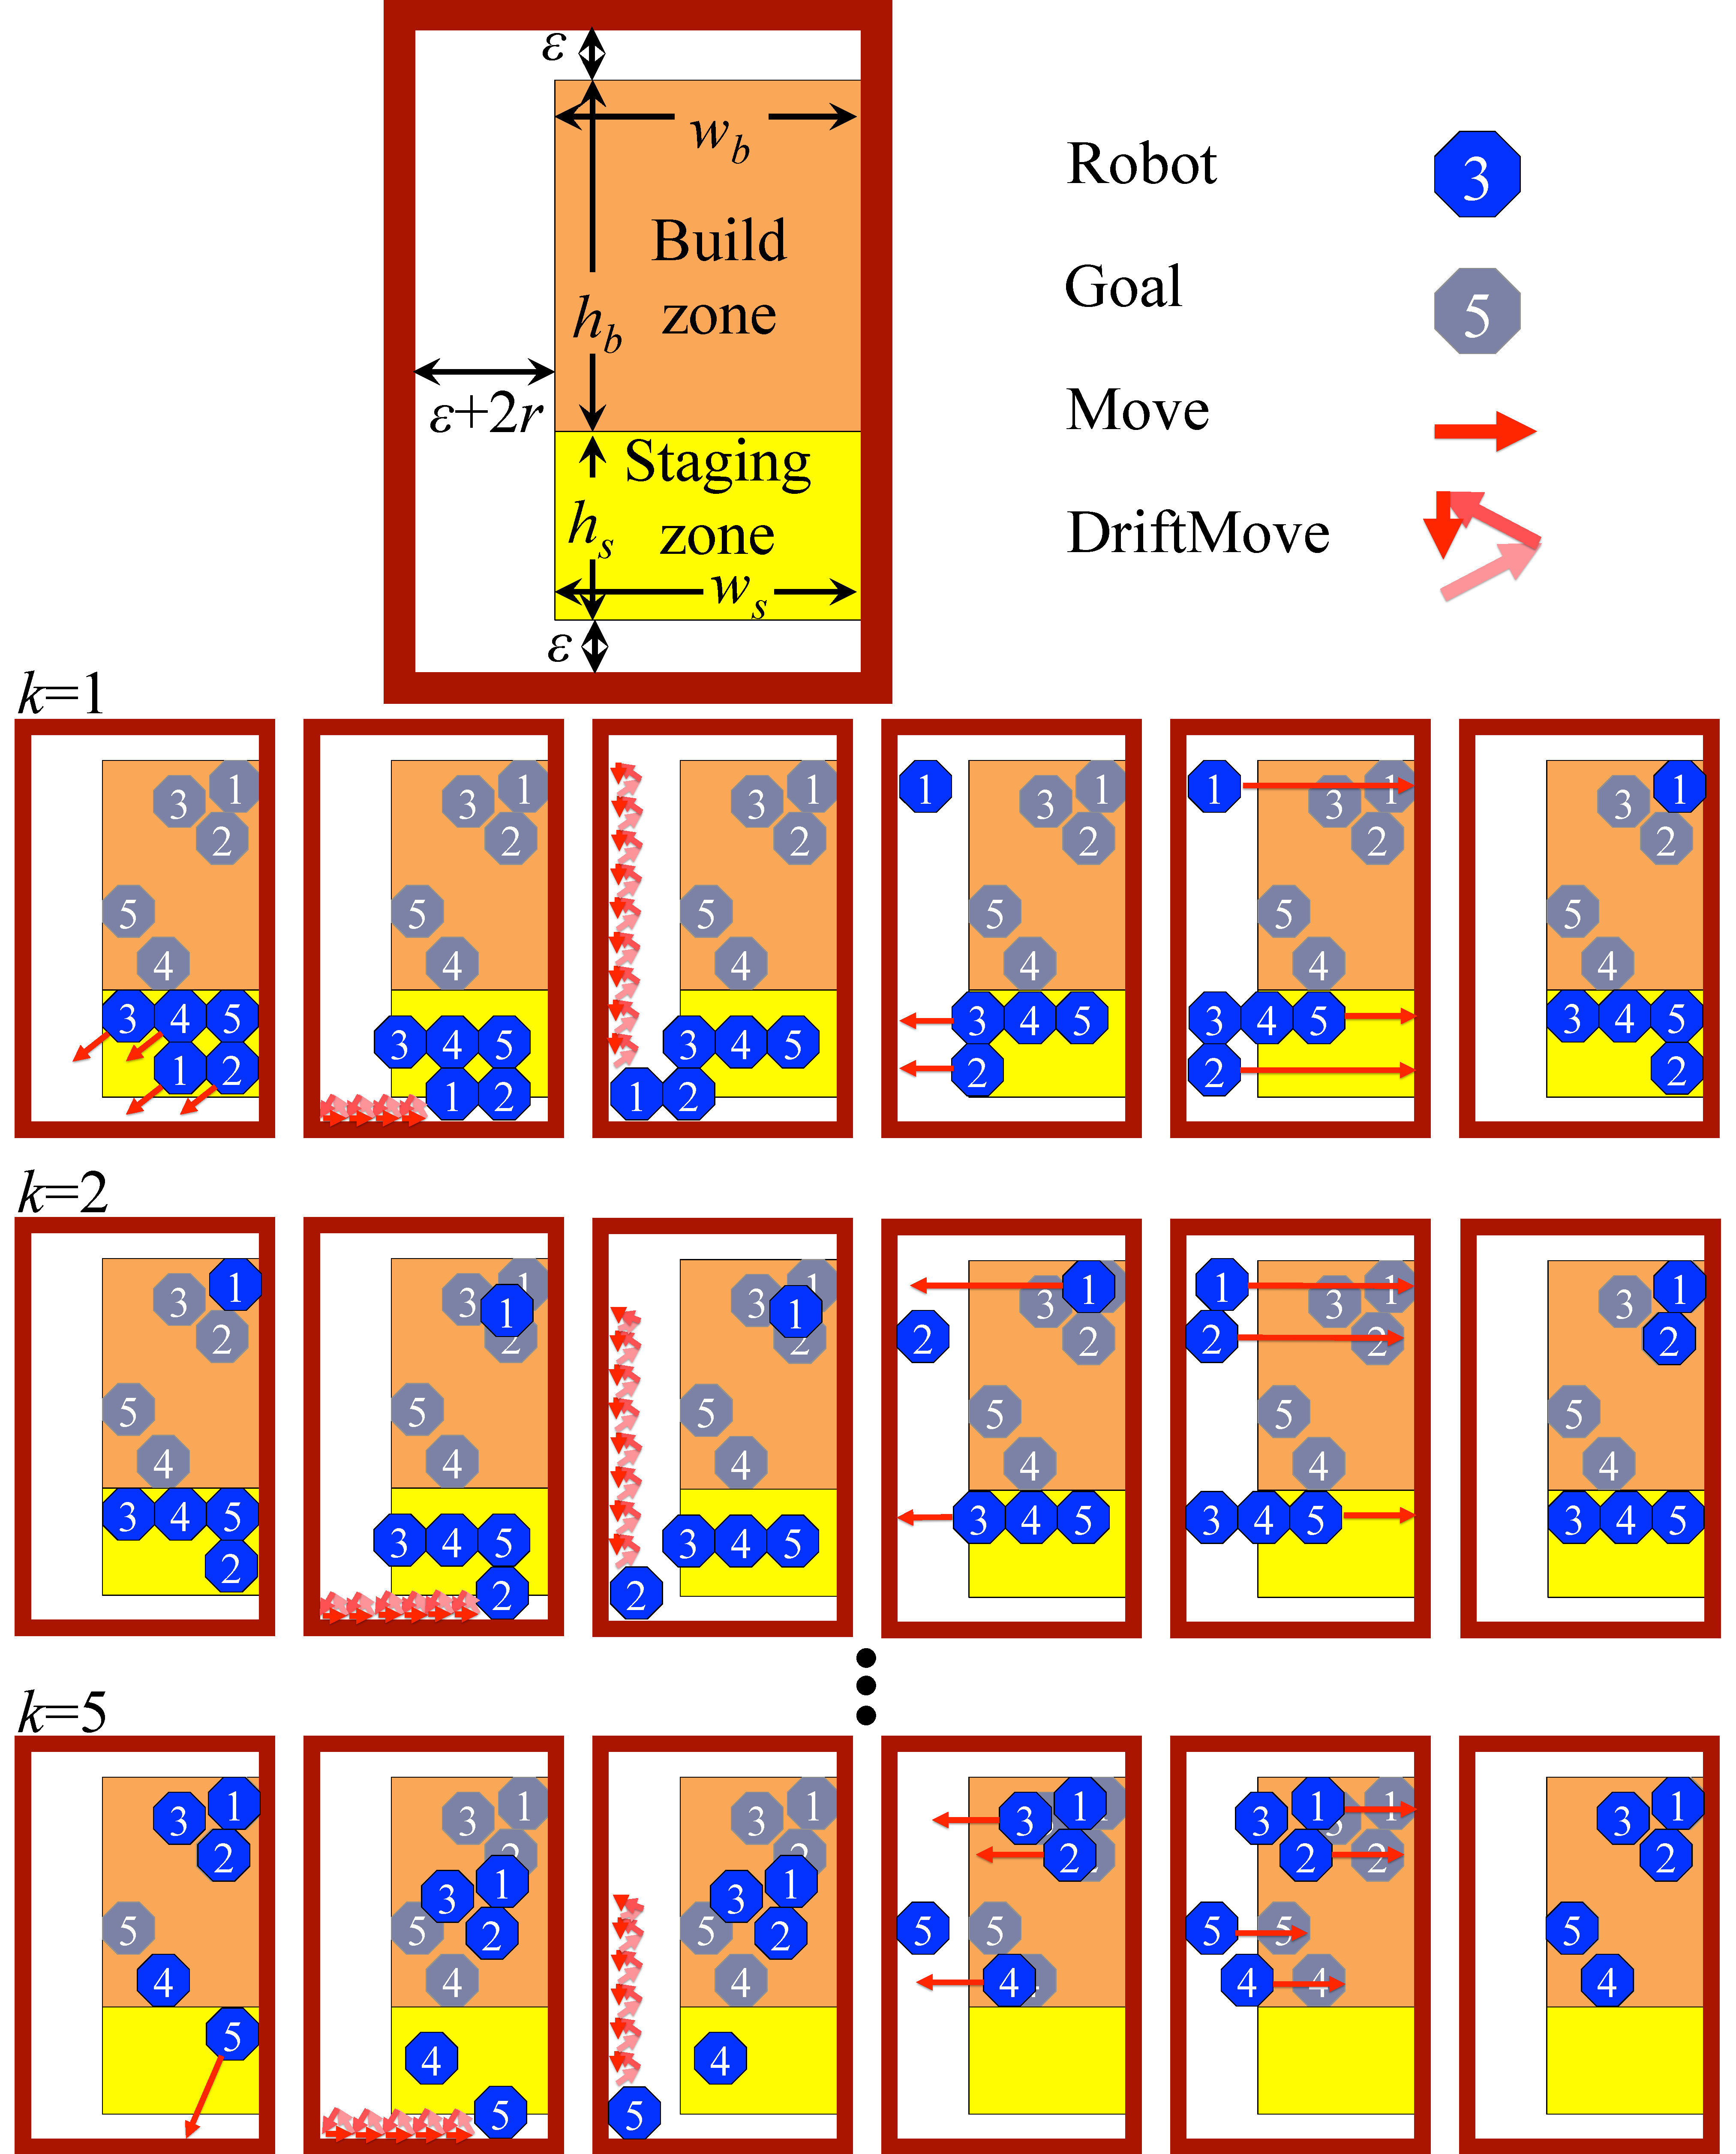
\includegraphics[width=1.0\columnwidth]{PositionNrobots.pdf}
\end{center}
\vspace{-1em}
\caption{\label{fig:construction2d}
Illustration of Alg.\ \ref{alg:PosControlNRobots}, $n$ robot position control  using wall friction.
}
\end{figure}




\subsection{AutomaticCovControl.mp4}
A closed-loop controller that steers a swarm of particles to a desired covariance,  implemented with a box2D simulator. In this video the green ellipse is the desired covariance ellipse, the red ellipse is the current covariance ellipse of the swarm and the red dot is the mean position of the robots. Robots follow the algorithm to achieve the desired values for $\sigma_{goalxy}$, $\sigma_x^2$ and $\sigma_y^2$.

%%%%%%%%%%%%%%%%%%%%%%%%%%%%%
\section{ Algorithm for generating desired $y$ spacing between two robots using wall friction}\label{sec:2robotWallFriction}
\begin{algorithm}
\caption{GenerateDesired$y$-spacing($s_1,s_2,e_1,e_2,L$)}\label{alg:YControl}
\begin{algorithmic}[1]
\Require Knowledge of starting $(s_1,s_2)$ and ending $(e_1,e_2)$ positions of  two robots. 
$(0,0)$ is bottom corner, $s_1$ is rightmost robot, 
 $L$ is length of the walls. Current position of the robots are $(r_1,r_2)$.
\Ensure   $ r_{1x} - r_{2x}  \equiv s_{1x} - s_{2x} $   %$\Delta y(t) \equiv \Delta y(0)$ 
\State $ \Delta s_y  \gets s_{1y} - s_{2y} $
\State $ \Delta e_y \gets e_{1y} - e_{2y} $
\State $ r_1 \gets s_1$, $ r_2 \gets s_2$
\If {$\Delta e_y < 0 $ }
\State $ m \gets ( L-\max( r_{1y},r_{2y}) ,0)   $ \Comment{Move to top wall}
\Else 
\State  $ m \gets ( -\min( r_{1y},r_{2y}),0 )    $ \Comment{Move to bottom wall}
\EndIf
\State $m  \gets  m + (0, -\min( r_{1x},r_{2x} ))$ \Comment{Move to left}
\State $ r_1 \gets r_1+m$, $ r_2 \gets r_2+m$ \Comment{Apply move}
\If {$\Delta e_y - (r_{1y} - r_{2y} ) > 0 $}
\State $ m \gets (\min(|\Delta e_y - \Delta s_y |, L- r_{1y}), 0)$  \Comment{Move top}
\Else
\State $ m \gets (-\min(|\Delta e_y - \Delta s_y |, r_{1y}), 0)$\Comment{Move bottom}
\EndIf 
\State $m  \gets  m + (0, \epsilon)$ \Comment{Move right}
\State $ r_1 \gets r_1+m$, $ r_2 \gets r_2+m$ \Comment{Apply move}
\State $\Delta r_y = r_{1y} - r_{2y}$
\If {$\Delta r_y \equiv \Delta e_y$} 
\State   $ m \gets (e_{1x}-r_{1x}, e_{1y}-r_{1y})$
\State $ r_1 \gets r_1+m$, $ r_2 \gets r_2+m$ \Comment{Apply move}
\State  \Return $(r_1,r_2)$
\Else   
\State \Return GenerateDesired$y$-spacing($r_1,r_2,e_1,e_2,L$)
\EndIf
\end{algorithmic}
\end{algorithm}



%%%%%%%%%%%%%%%%%%%%%%%%%%%
\section{Calculations for modeling swarm as fluid in a simple planar workspace}\label{sec:fluidInPlanarRegion}
Two workspaces are used, a square and a circular workspace.

\subsection{Square Workspace}
This section provides formulas for the mean, variance,  covariance and correlation of a very large swarm of robots as they move inside a square workplace under the influence of gravity pointing in the direction $\beta$. The swarm is large, but the robots are small in comparison, and together cover an area of constant volume $A$. Under a global input such as gravity, they flow like water, moving to a side of the workplace and forming a polygonal shape. The workspace is 

The range of possible angles for the global input angle $\beta $ is [0,2$\pi $). In this range of angles, the swarm assumes eight different polygonal shapes. The shapes alternate between triangles and trapezoids when the area $A$$<$1/2, and alternate between squares with one corner removed and trapezoids when $A$$>$1/2.

Two representative formulas are attached, the outline of the swarm shapes in \eqref{tab:SquareRobotRegions} and $\bar{x}(\beta,A)$ in \eqref{tab:SquareXMean}.




\begin{figure}[h]
\begin{center}
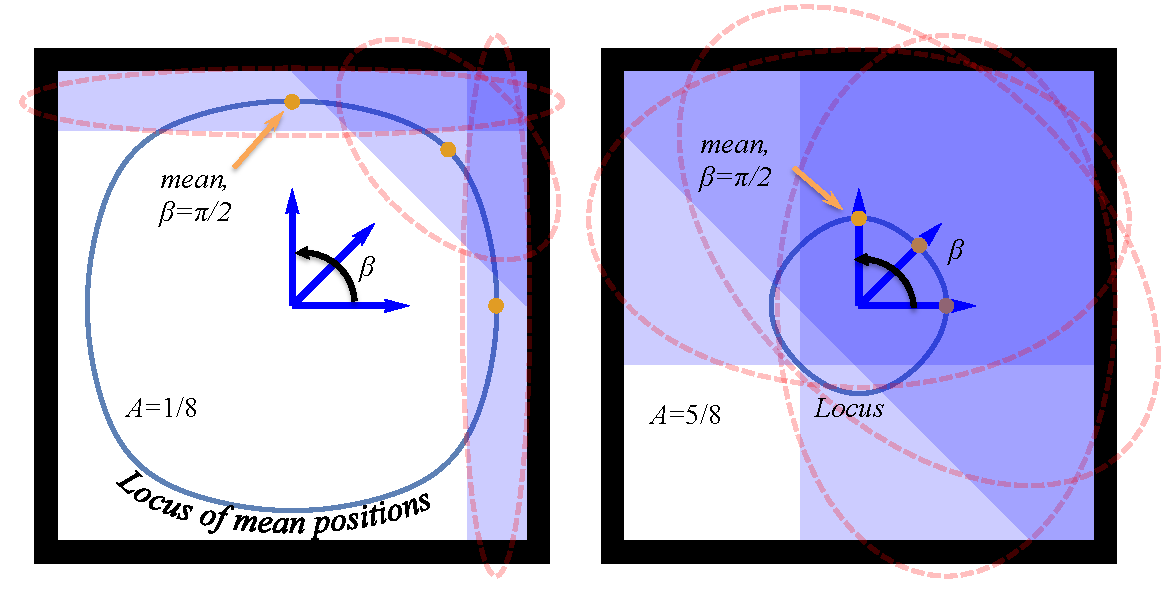
\includegraphics[width=\columnwidth]{SquarePlotPositions.pdf} 
\caption{A swarm in a square workspace under a constant global input assumes either a triangular or a trapezoidal shape if $A<1/2$.  If $A>1/2$ the swarm is either a squares with one corner removed or a trapezoidal  shape.}
\label{fig:friction}
\end{center}
\end{figure} 

\begin{table*}
\begin{align}
\bar{x}(\beta,A) = A\leq \frac{1}{2}: &\begin{cases}
 -\frac{\tan ^2(\beta )}{24 A}-\frac{A}{2}+1 & 0\leq \beta \leq \tan ^{-1}(2 A)\lor 2 \pi -\tan ^{-1}(2 A)<\beta \leq 2 \pi  \\
 1-\frac{1}{3} \sqrt{2} \sqrt{A \tan (\beta )} & \tan ^{-1}(2 A)<\beta \leq \frac{\pi }{2}-\tan ^{-1}(2 A) \\
 \frac{\cot (\beta )}{12 A}+\frac{1}{2} & \frac{\pi }{2}-\tan ^{-1}(2 A)<\beta \leq \tan ^{-1}(2 A)+\frac{\pi }{2} \\
 \frac{1}{3} \sqrt{2} \sqrt{-A \tan (\beta )} & \tan ^{-1}(2 A)+\frac{\pi }{2}<\beta \leq \pi -\tan ^{-1}(2 A) \\
 \frac{\tan ^2(\beta )}{24 A}+\frac{A}{2} & \pi -\tan ^{-1}(2 A)<\beta \leq \tan ^{-1}(2 A)+\pi  \\
 \frac{1}{3} \sqrt{2} \sqrt{A \tan (\beta )} & \tan ^{-1}(2 A)+\pi <\beta \leq \frac{3 \pi }{2}-\tan ^{-1}(2 A) \\
 \frac{1}{2}-\frac{\cot (\beta )}{12 A} & \frac{3 \pi }{2}-\tan ^{-1}(2 A)<\beta \leq \tan ^{-1}(2 A)+\frac{3 \pi }{2} \\
 1-\frac{1}{3} \sqrt{2} \sqrt{-A \tan (\beta )} & \tan ^{-1}(2 A)+\frac{3 \pi }{2}<\beta \leq 2 \pi -\tan ^{-1}(2 A) \\
\end{cases} \nonumber\\
\frac{1}{2}<A<1:&\begin{cases}
 -\frac{\tan ^2(\beta )}{24 A}-\frac{A}{2}+1 & 0\leq \beta \leq \tan ^{-1}\left(\frac{1}{2},1-A\right)\lor 2 \pi -\tan ^{-1}\left(\frac{1}{2},1-A\right)<\beta \leq 2 \pi  \\
 \frac{2 \sqrt{2} \sqrt{(1-A) \tan (\beta )} (A-1)+3}{6 A} & \tan ^{-1}\left(\frac{1}{2},1-A\right)<\beta \leq \frac{\pi }{2}-\tan ^{-1}\left(\frac{1}{2},1-A\right) \\
 \frac{6 A+\cot (\beta )}{12 A} & \frac{\pi }{2}-\tan ^{-1}\left(\frac{1}{2},1-A\right)<\beta \leq \tan ^{-1}\left(\frac{1}{2},1-A\right)+\frac{\pi }{2} \\
 \frac{-2 \sqrt{2} \sqrt{(A-1) \tan (\beta )} (A-1)+6 A-3}{6 A} & \tan ^{-1}\left(\frac{1}{2},1-A\right)+\frac{\pi }{2}<\beta \leq \pi -\tan ^{-1}\left(\frac{1}{2},1-A\right) \\
 \frac{\tan ^2(\beta )}{24 A}+\frac{A}{2} & \pi -\tan ^{-1}\left(\frac{1}{2},1-A\right)<\beta \leq \tan ^{-1}\left(\frac{1}{2},1-A\right)+\pi  \\
 \frac{2 \sqrt{2} \sqrt{(1-A) \tan (\beta )} (1-A)+6 A-3}{6 A} & \tan ^{-1}\left(\frac{1}{2},1-A\right)+\pi <\beta \leq \frac{3 \pi }{2}-\tan ^{-1}\left(\frac{1}{2},1-A\right) \\
 \frac{1}{2}-\frac{\cot (\beta )}{12 A} & \frac{3 \pi }{2}-\tan ^{-1}\left(\frac{1}{2},1-A\right)<\beta \leq \tan ^{-1}\left(\frac{1}{2},1-A\right)+\frac{3 \pi }{2} \\
 \frac{2 \sqrt{2} \sqrt{(A-1) \tan (\beta )} (A-1)+3}{6 A} & \tan ^{-1}\left(\frac{1}{2},1-A\right)+\frac{3 \pi }{2}<\beta \leq 2 \pi -\tan ^{-1}\left(\frac{1}{2},1-A\right) \\
\end{cases}
 \nonumber \\
A=1: &\frac{1}{2}
\end{align}
\protect\caption{$\bar{x}$ in a unit-square workspace}
\label{tab:SquareXMean}
\end{table*}



\begin{table*}
\tiny
\begin{align}
\text{RobotRegion}(\beta,A)= \nonumber 
A\leq \frac{1}{2}:&
\begin{cases}
 \left(
\begin{array}{cc}
 1 & 0 \\
 1 & 1 \\
 -A-\frac{\tan (\beta )}{2}+1 & 1 \\
 -A+\frac{\tan (\beta )}{2}+1 & 0 \\
\end{array}
\right) & 0\leq \beta \leq \tan ^{-1}(2 A)\lor 2 \pi -\tan ^{-1}(2 A)<\beta \leq 2 \pi  \\
 \left(
\begin{array}{cc}
 1 & 1 \\
 1-\sqrt{2} \sqrt{A \tan (\beta )} & 1 \\
 1 & 1-\sqrt{2} \sqrt{A \cot (\beta )} \\
\end{array}
\right) & \tan ^{-1}(2 A)<\beta \leq \frac{\pi }{2}-\tan ^{-1}(2 A) \\
 \left(
\begin{array}{cc}
 1 & 1 \\
 0 & 1 \\
 0 & -A+\frac{\cot (\beta )}{2}+1 \\
 1 & -A-\frac{\cot (\beta )}{2}+1 \\
\end{array}
\right) & \frac{\pi }{2}-\tan ^{-1}(2 A)<\beta \leq \tan ^{-1}(2 A)+\frac{\pi }{2} \\
 \left(
\begin{array}{cc}
 0 & 1 \\
 \sqrt{2} \sqrt{-A \tan (\beta )} & 1 \\
 0 & 1-\sqrt{2} \sqrt{-A \cot (\beta )} \\
\end{array}
\right) & \tan ^{-1}(2 A)+\frac{\pi }{2}<\beta \leq \pi -\tan ^{-1}(2 A) \\
 \left(
\begin{array}{cc}
 0 & 0 \\
 0 & 1 \\
 A-\frac{\tan (\beta )}{2} & 1 \\
 A+\frac{\tan (\beta )}{2} & 0 \\
\end{array}
\right) & \pi -\tan ^{-1}(2 A)<\beta \leq \tan ^{-1}(2 A)+\pi  \\
 \left(
\begin{array}{cc}
 0 & 0 \\
 0 & \sqrt{2} \sqrt{A \cot (\beta )} \\
 \sqrt{2} \sqrt{A \tan (\beta )} & 0 \\
\end{array}
\right) & \tan ^{-1}(2 A)+\pi <\beta \leq \frac{3 \pi }{2}-\tan ^{-1}(2 A) \\
 \left(
\begin{array}{cc}
 0 & 0 \\
 1 & 0 \\
 1 & A-\frac{\cot (\beta )}{2} \\
 0 & A+\frac{\cot (\beta )}{2} \\
\end{array}
\right) & \frac{3 \pi }{2}-\tan ^{-1}(2 A)<\beta \leq \tan ^{-1}(2 A)+\frac{3 \pi }{2} \\
 \left(
\begin{array}{cc}
 1 & 0 \\
 1-\sqrt{2} \sqrt{-A \tan (\beta )} & 0 \\
 1 & \sqrt{2} \sqrt{-A \cot (\beta )} \\
\end{array}
\right) & \tan ^{-1}(2 A)+\frac{3 \pi }{2}<\beta \leq 2 \pi -\tan ^{-1}(2 A) \\
\end{cases}
 %%%%%%%%%%%%%%%%%%%%%%%%%%%%%%%%%%
\nonumber \\
\frac{1}{2}<A<1:&
\begin{cases}
 \left(
\begin{array}{cc}
 1 & 0 \\
 1 & 1 \\
 (1-A)-\frac{\tan (\beta )}{2} & 1 \\
 (1-A)+\frac{\tan (\beta )}{2} & 0 \\
\end{array}
\right) & 0\leq \beta \leq \tan ^{-1}\left(\frac{1}{2},1-A\right)\lor 2 \pi -\tan ^{-1}\left(\frac{1}{2},1-A\right)<\beta \leq 2 \pi  \\
 \left(
\begin{array}{cc}
 1 & 0 \\
 1 & 1 \\
 0 & 1 \\
 0 & \sqrt{2} \sqrt{(1-A) \cot (\beta )} \\
 \sqrt{2} \sqrt{(1-A) \tan (\beta )} & 0 \\
\end{array}
\right) & \tan ^{-1}\left(\frac{1}{2},1-A\right)<\beta \leq \frac{\pi }{2}-\tan ^{-1}\left(\frac{1}{2},1-A\right) \\
 \left(
\begin{array}{cc}
 0 & 1 \\
 1 & 1 \\
 1 & (1-A)-\frac{\cot (\beta )}{2} \\
 0 & (1-A)+\frac{\cot (\beta )}{2} \\
\end{array}
\right) & \frac{\pi }{2}-\tan ^{-1}\left(\frac{1}{2},1-A\right)<\beta \leq \tan ^{-1}\left(\frac{1}{2},1-A\right)+\frac{\pi }{2} \\
 \left(
\begin{array}{cc}
 1 & 1 \\
 0 & 1 \\
 0 & 0 \\
 1-\sqrt{2} \sqrt{-(1-A) \tan (\beta )} & 0 \\
 1 & \sqrt{2} \sqrt{-(1-A) \cot (\beta )} \\
\end{array}
\right) & \tan ^{-1}\left(\frac{1}{2},1-A\right)+\frac{\pi }{2}<\beta \leq \pi -\tan ^{-1}\left(\frac{1}{2},1-A\right) \\
 \left(
\begin{array}{cc}
 0 & 0 \\
 0 & 1 \\
 -(1-A)-\frac{\tan (\beta )}{2}+1 & 1 \\
 -(1-A)+\frac{\tan (\beta )}{2}+1 & 0 \\
\end{array}
\right) & \pi -\tan ^{-1}\left(\frac{1}{2},1-A\right)<\beta \leq \tan ^{-1}\left(\frac{1}{2},1-A\right)+\pi  \\
 \left(
\begin{array}{cc}
 1 & 0 \\
 0 & 0 \\
 0 & 1 \\
 1-\sqrt{2} \sqrt{(1-A) \tan (\beta )} & 1 \\
 1 & 1-\sqrt{2} \sqrt{(1-A) \cot (\beta )} \\
\end{array}
\right) & \tan ^{-1}\left(\frac{1}{2},1-A\right)+\pi <\beta \leq \frac{3 \pi }{2}-\tan ^{-1}\left(\frac{1}{2},1-A\right) \\
 \left(
\begin{array}{cc}
 1 & 0 \\
 0 & 0 \\
 0 & -(1-A)+\frac{\cot (\beta )}{2}+1 \\
 1 & -(1-A)-\frac{\cot (\beta )}{2}+1 \\
\end{array}
\right) & \frac{3 \pi }{2}-\tan ^{-1}\left(\frac{1}{2},1-A\right)<\beta \leq \tan ^{-1}\left(\frac{1}{2},1-A\right)+\frac{3 \pi }{2} \\
 \left(
\begin{array}{cc}
 0 & 0 \\
 1 & 0 \\
 1 & 1 \\
 \sqrt{2} \sqrt{-(1-A) \tan (\beta )} & 1 \\
 0 & 1-\sqrt{2} \sqrt{-(1-A) \cot (\beta )} \\
\end{array}
\right) & \tan ^{-1}\left(\frac{1}{2},1-A\right)+\frac{3 \pi }{2}<\beta \leq 2 \pi -\tan ^{-1}\left(\frac{1}{2},1-A\right) \\
\end{cases},\nonumber\\
%%%%%%%%%%%%%%%%%%%%%%%%%%%%%%%
A=1:&\left(
\begin{array}{cc}
 1 & 0 \\
 0 & 0 \\
 0 & 1 \\
 1 & 1 \\
\end{array}
\right)
\end{align}
\protect\caption{RobotRegions in a unit-square workspace}
\label{tab:SquareRobotRegions}
\end{table*}


\subsection{Circle Workspace}
The area under a chord of a circle is the area of a sector less the area of the triangle originating at the circle center: 
$A=S(sector)-S(triangle)=1/2 LR-1/2 C(1-h)$, thus
\begin{align}
A=(1/2)\left[LR-c(R-h)\right]
\end{align}
where $L$ is arc length, $c$ is chord length, $R$ is radius and $h$ is height. Solving for $L$ and $C$ gives
\begin{align}
L&=2 \cos ^{-1}(1-h)\\
C&=2\sqrt{h(2-h)}
\end{align}
Therefore the area under a chord is
\begin{align}
\cos ^{-1}(1-h)-(1-h) \sqrt{(2-h) h}
\end{align}

For a circular workspace, with $\beta = 0$, the variance of $x$ and $y$ are:
{\tiny
\begin{align}
&\sigma_x^2(h)=\frac{64 (h-2)^3 h^3}{144 \left(\sqrt{-(h-2) h} (h-1)+\arccos(1-h)\right)^2} +\nonumber\\
&\frac{9 \left(\sqrt{-(h-2) h} (h-1)+\arccos(1-h)\right) \left(\sin \left(4 \arcsin(1-h)\right)+4 \arccos(1-h)\right)}{144 \left(\sqrt{-(h-2) h} (h-1)+\arccos(1-h)\right)^2}
\end{align}}

{\tiny
\begin{align}
\sigma_y^2(h)=
\frac{12 \arccos(1-h)-8 \sin \left(2 \arccos(1-h)\right)+\sin \left(4 \arccos(1-h)\right)}{48 \left(\sqrt{-(h-2) h} (h-1)+\arccos(1-h)\right)}
\end{align}}

For $\beta = 0$, $\sigma_{xy}=0$. These values can be rotated to calculate $\sigma_x^2(\beta,h),\sigma_y^2(\beta,h),$ and $\sigma_{xy}(\beta,h)$.

%%%%%%%%%%%%%%%%%%%%%%%%%%%%%%
\section*{Acknowledgments}
This work was supported by the National Science Foundation under Grant No.\ \href{http://nsf.gov/awardsearch/showAward?AWD_ID=1553063}{ [IIS-1553063]}.

%%%%%%%%%%%%%%%
%% Use plainnat to work nicely with natbib. 
\bibliographystyle{plainnat}
\footnotesize
\bibliography{IEEEabrv,ShapingSwarmFrictionSharedInput}
\end{document}





\end{document}